\documentclass[10pt]{article}
%\usepackage{fullpage}
%\usepackage[top=1in,bottom=1in,left=1in,right=1in]{geometry}
\usepackage{courier}
\usepackage{color}
\usepackage{url}
\usepackage{graphicx}
\newcommand{\PROBLEM}[1] {\textbf{\textcolor{red}{#1}}}

\title{Active RDMA}
\author{Chris Fallin, Anshul Madan, Filipe Milit\~{a}o\\ \\
15-712: Advanced Operating Systems \&  Distributed Systems\\
Carnegie Mellon University}
\date{}
\begin{document}

\maketitle

\begin{abstract}
A classic functionality tradeoff exists between client and server in a
distributed system such as a network filesystem. One approach, widely
used, is to define a static API at the server and allow RPCs to this
API from clients. This approach allows the server implementation to be
optimized for these specific operations. An alternate proposal,
RDMA~\cite{thekkath94}, proposes to allow direct remote memory access
in order to reduce latency and increase flexibility by exposing data
structures directly. However, this approach can suffer from a lack of
performance because code is widely separated from the data on which it
operates. In this project, we propose and prototype a middle ground,
\emph{Active RDMA}, that uses code migration to enable data-code
locality while retaining the flexibility of the RDMA approach. We
propose to run the \emph{active code} directly on the NIC, with full
access to host memory. We modify a full-system simulator and use this
infrastructure to build a proof-of-concept network filesystem, and
provide an initial evaluation of the concept.

\end{abstract}

\section{Introduction}

Traditional distributed services have built upon RPC or RPC-like
interfaces at the network level. In these systems, a server exports a
static set of operations, typically at a high level. For example, a
file server allows a client to open a file in one call, and read a
block of data in the next. An alternate paradigm exists: RDMA (Remote
Direct Memory Access), first proposed in~\cite{thekkath94}, exposes
data structures in the server's memory directly. Client applications
can then, with knowledge of the appropriate structures, implement most
intelligence on the client side and access shared data remotely. The
advantage of this scheme is that it allows low-latency operation if
the RDMA mechanism is implemented efficiently (i.e., in hardware or at
the low level in a system software trap). It also allows more
flexibility in client operations by allowing a finer granularity than
a static high-level API, although this aspect was not evaluated in the
original proposal. The disadvantage is that, for complex
data-structure manipulations or pathological cases (e.g., a long
linked list in memory), the cost of multiple round-trips over the
network can be extreme compared to performing the computation locally
at the server.

We attempt to retain the benefits of both designs by building a
hybrid. In the spirit of Active Networks~\cite{AN-survey}, we propose
to allow clients to send code to the server to execute directly
against the shared data structures. We call this \textbf{Active
  RDMA}. This functionality will allow for the \emph{flexibility} and
\emph{client-driven intelligence} of RDMA while providing the
\emph{data locality} advantages of traditional server-side code.

In order to narrow the scope of our project, we focus specifically on
environments in which security is not an explicit concern. This seems
strange at first in the context of a network-centric project, but
such environments do exist. For example, large computing clusters or
datacenters with a single owner, in which all machines or network
devices are trusted and performance is the paramount concern, are one
possible application domain.

Furthermore, the assumption that security is externally provided
(whole-cluster access control) or otherwise an orthogonal problem
allows us to push Active RDMA's code execution to a lower level,
bypassing layers for higher performance. 

We define our interface to be sufficiently low-level that it could
hypothetically execute directly on a network interface
card~\cite{nic-basedreduction}, interacting with shared memory via
DMA.  This would allow for extremely low latency.

A secondary benefit to this, and one that we explore, lies in the
flexibility of executing arbitrary code segments on the server,
defined by an application. For example, a ``grep''-like operation to
search through some shared data structure might be significantly
faster when executed on the server than when querying a fixed
interface from the client side. (In practice, our ``grep'' was not
optimized enough relative to the system {\tt grep(1)} to show an
actual improvement, but the concept appears sound nonetheless.)

Our work consists of several main contributions:

\begin{itemize} \itemsep -2pt

\item Defining a low-level interface for remote code based on Java
  class-file shipping and both word-level and byte-level shared memory
  access; defining a protocol and building reference implementations
  of a server and a client library to enable use of this ActiveRDMA
  interface.

\item Building a simulation infrastructure to examine the performance
  tradeoffs of the performance split. We base this infrastructure on a
  conglomeration of the Bochs x86 simulator and the standard Java JVM
  with a timing model, in order to give some level of fidelity
  (however coarse) to our comparison results.

\item Building a distributed file system on top of this
  infrastructure, keeping data in-memory for simplicity, and
  evaluating against NFS; showing use of code shipping to optimize
  \emph{grep} and \emph{find}.

\end{itemize}

\section{Background and Related Work}

As discussed above, the primary advantage of a basic RDMA system is
that there is low latency for common data-transfer operations that
require little actual logic on the server side, and deal with simple
data structures. However, the inability to execute code on the server
can lead to unacceptably high cost for some common operations, such as
a linked list traversal. The proposal in~\cite{thekkath94} gets around
this limitation by also allowing RPC in some cases (e.g., when their
nameserver implementation cannot find an entry after a certain number
of hash-table probes). This is a win for performance, but then
eliminates the flexibility that client-side logic has for
application-specific optimizations. Our Active RDMA idea retains this
flexibility while attempting to regain some of the server-side
performance.

Our work differs in several ways from previous work and other
alternatives:

\begin{itemize} \itemsep -2pt

\item Active Networks are primarily proposed for customization at the
  network or routing layer: for example, upgrading TCP~\cite{AN-tcp},
  or providing programmable packet-forwarding as in ANTS~\cite{ANTS},
  PLANet~\cite{planet} or FIRE~\cite{FIRE}.

\item Active Disks~\cite{AD2,AD} execute code at a disk controller,
  increasing data locality for certain types of data preprocessing in
  the same way as Active RDMA will allow for storage applications.
  However, Active Disks are limited in scope to this data processing.
  In contrast, Active RDMA is a generic mechanism that not only will
  allow for storage applications but any distributed system that
  requires some shared state at a central server. Also, the fact the
  interface would allow the RDMA code to be executed on the NIC itself, 
  should improve the performance of network storage applications.

\item Mobile code~\cite{mobile} is the name for a general research
  thrust of code migration over networks in order to build distributed
  systems. This is the most similar to our idea. However, mobile
  code is generally a higher-level abstraction that does not provide
  direct access to a shared memory segment, for example, and provides
  more sandboxing and security that remove many of the potential
  performance benefits that we are aiming for. We also do not plan for any kind of special language integration and instead rely on traditional interfaces and Java bytecode gets send directly through the network.

\end{itemize}

\section{Implementation}

%So far, we have built a prototype implementation of Active RDMA in
%Java, as well as several simple test applications, and we plan to move
%onto a full system simulator-based evaluation framework and a
%FUSE-based client filesystem interface so that we can more accurately
%evaluate performance. Our progress can be summarized by
%these accomplishments so far:

We developed a prototype implementation of Active RDMA with the goal of having both a reference implementation of our concept and also to use it to provide significant test results to either prove or disprove our beliefs of performance gains. As with any proof-of-concept code, it does not aim to be full feature and it makes some strong assumptions (such as result sizes, packet formats, etc) to reduce the complexity of the code and allow us to reach the testing phase quicker. We based our implementation on the Java programming language for convenience of the development tools and the flexibility of the JVM in dealing with the uploaded code.

The most crucial point of our implementation is the definition of the Active RDMA client-server interface, both at the API level and at the wire protocol level, since it needs to be simple and small but powerful enough to facilitate efficient use of the server's resources. The interface allows direct memory
  access as well as code migration (using Java bytecode), and supports
  the following basic operations:
  \begin{itemize}
  \item {\tt Read}, {\tt Write}, {\tt Compare-and-Swap} -- as in original RDMA, these
    allow for direct memory access over the network but both {\tt read}
    and {\tt write} operations are defined over blocks of addresses (so
    that batching is possible) which allows us to group together multiple similar requests in the same packet.
  \item {\tt Load(bytecode)} -- loads a Java class file into the remote
    environment. This will cause the class' byte code to be sent over the wire and loaded on the server side. The code is then indexed using an MD5 hash to detect code duplication and disambiguate between multiple version of the same class code (although limitations on the JVM forbid us of having more than one class with a given name and we did not have time to play around with tools to modify the uploaded bytecode to circumvent this). 
    
    For this implementation we used a fixed format for the method signature:
    
    {\tt \textbf{public static int}[] execute(ActiveRDMA a, \textbf{int}[] args)}

Although, for convenience, we also allow:

    {\tt \textbf{public static int} execute(ActiveRDMA a, \textbf{int}[] args)}

(where the result gets wrapped in an array so that the semantics remain identical to the previous one). This signatures allows for the code, when it is run on the server, to be used in exactly the same way as when it is run from a RDMA only perspective (that is, a client interface that sends all those basic requests across the network to the server). 

  \item {\tt Execute(code, param)} -- Executes previously-loaded remote code
    (referenced by MD5 hash), giving it direct access to the host
    memory. Both \textit{param} and the result can use arrays of integers so that more complex arguments and results can be required/produced by an execution although more complex types (such as strings) need to be converted to/from their internal representation into an array of ints.
     
  \end{itemize}
  
  This simple interface also includes a series of error codes to account for common mistakes that may occur during execution such as going beyond the memory bounds of the server. We also defined a series of more complex operations that use this simple interface as building block or that are just more convenient for the programmer to use (like just passing a class to the load function instead of having to manually extract its byte code). 
Finally, even if this was not thoroughly explored, we could also have defined a set of useful library functions for memory management or other convenient procedures that are necessary in real-world production environments.
  
   The server consists of a single large array representing host memory and
  an implementation of the wire protocol and Java environment (class
  loader, etc). The client consists of a library that allows the user
  to easily load classes and call them remotely. We based our wire protocol on UDP packets specially to simplify the modification of the test virtual machine (so that it did not require the implementation of a full TCP network stack). This means we made certain assumption of the packet size to keep failure handling simple (in this case a simple timeout and resend).
  The execution model on the server side is also meant to be simple: a fixed number of threads listens to jobs that are pushed into a single work queue. If a job waits for to long to be handle, it is just assumed to have expired and is ignored. Traditional RDMA request are handled immediately as they should be fairly lightweight and not cause any abuse in the use of server's resources. As a consequence of this execution architecture, we could have situation where an expensive computation ends up running multiple times due to response timeouts on the client side. We did not handle such case as well as providing more control over what computational resources the active code is allowed to use. However, the first case can be handled easily by just pushing some complexity to the active code that needs to have a ``guard'' memory position to tracks the state of the computation (such as ``not-stated'', ``running'' and ``done''). Before starting the heavy code, it just checks to ensure that there is no previously ``running'' or ``done'' values (using compare and swap to avoid races).

\subsection{Initial demo applications}

We built four simple demo application using our prototype framework. 
\begin{itemize}
\item linked list - where the most significant operation (from the cost perspective) is the insertion operation as it needs to iterate across all elements of that list before if can insert a new element at the end.
\item hash table - again where the insertion operation represents the most significant cost, as it has the potential to require multiple lookups before it finds an item.
\item in-memory filesystem (built using the hash table).
\item locking (mutual exclusion) service with FCFS lock ordering~\cite{nic-basedatomic}.  
\end{itemize}

Running the first two as both plain RDMA and as Active code served as initial benchmarks whose results encouraged us to continue with the implementation. The results of running in a local machine (where network latency and bandwidth should be considerably smaller than any real remote execution), are shown in Figure \ref{res1}.

\begin{figure}[h!]
\center
\begin{tabular}{|ccc|}
\hline
Algorithm & Operation & Run Time\\
\hline
list - RDMA &  put & 39.675 ms \\
list - RDMA & get & 19.38 ms \\
\hline
list - Active & put & 0.33 ms \\
list - Active & get & 0.245 ms \\
\hline
\hline
table - RDMA  & put & 1.919 ms\\
table - RDMA   & get & 1.739 ms\\
\hline
table - Active  &put & 0.245 ms\\
table - Active & get & 0.239 ms\\
\hline
\end{tabular}
\caption{Results for RDMA and Active operations on a list and hash table.}
\label{res1}
\end{figure}

These results show gains consistent with the complexity of the operation. Thus, the insertion of 200 elements in a list as well as the iteration over all those elements has a considerable gain on the Active version when compared with the RDMA version that requires all requests to be sent over the wire. On the hash-table side, gains were still significant but more modest as this structure has a lower computational complexity both for insertion and access and therefore, will pay a lower performance penalty for using the network. 

The last two application (the file system and the locking service), were then extended into the full testing framework discussed further below.

\subsection{Active RDMA File System Server}

The core of the testing framework is centered on an in-memory file system that is accessible through the Active RDMA interface and uses the DHT for managing directory entries. It is not meant to be a complete FS and instead is just a core implementation of the basic FS functionalities needed to test our approach. It supports batch reads and writes but the file is restricted to a fixed size and therefore, any append that goes beyond the file's limit must copy the old content to the new location. This pushes some complexity to the application but achieves great simplicity in the implementation by making all content accessible in a contiguous block.

The following Active DFS operations were implemented : create, lookup, getBlock, setBlock, setLen, getLen, read, write, copy, find. the implementation ensures a single rountrip for each Active DFS operation which is the core strenght of the Avtive RDMA protocol.

For example, the Active DFS implementation uses other Active code like DHT as a library. In out implementation, using run() we send a request to the server to execute particular Active Code, which internally may call other Active code from libraries which are also loaded on the server beforehand. Thus Active RDMA DFS ensures that there are never more than a single round trip between client and server when a single operations is executed. 


\subsection{Active RDMA File System Client}

The Active DFS client is implemented as a FUSE file system, which considerably simplifies the development effort for us. We used JNI bindings to implement the Active DFS client code in java. Java Native Interface (JNI) is a programming framework that allows Java code running in a Java Virtual Machine (JVM) to call and to be called[1]  by native applications (programs specific to a hardware  and operating system platform) and libraries written in other languages, such as C. Our implementation has been built on top of the FUSE J code, which is freely available on sourceforge.net. The FileSystem3 is an adapter interface that is eventually called by the linux system calls. Our file system called ARFS(Active RDMA FIle system) basically implements this interface, by using the Active RDMA wire interface to generate packets sent over the wire, or using libraries we implemented like List, DHT that eventually send packets over the wire using the Active RDMA wire transfer interface. We have supported a file system interface that very closely emulates that of a linux file system calls, because these are required to accurately measure the performance of ARFS.


\subsection{DFS utilities (Grep, Copy and Find)}

In order to use the file system and expose our performance gains, we built the following utilities that make use of the higher level file system interface:

\begin{itemize}
\item Copy -- a simple utility that is able of copying a file already in DFS to a new position as well as pinning a file in the systems' filesystem to DFS (that is, transfer a file to memory). The expected performance gains are mostly due to keeping all transfers locally instead of having to move each chunk across the network (on a read) just to be written in another block (on a write) on the server side.

\item Grep -- does simple pattern matching on a text file. It takes a regular expression that is then used to filter a text file and returns all lines that contain that expression. Although we did not experiment with more dynamic code generation (that would truly expose the advantage of such dynamic system), our prototype implementation of this utility should be enough to serve as proof-of-concept that our model can achieve significant performance gains when compared with purely client side RDMA even if a static code migration mechanism (such as in traditional RPC) could also be used in such heavily constrained scenario to get similar benefits. Thus, we leave as future work the potential to send dynamically generated code that matches the data-structures on the server side more efficiently, instead of sending the pattern that gets used in a generic pattern matcher. 
We made an assumption that the result will necessarily fit into a single packet and as such our tests have been design with this limitation in mind.

\item Find -- this utility searches for files that match a specific name pattern. It essentially just traverses the directory table selecting all entries that have compatible names. We did not use the same size restriction as on the previous utility and instead rely on basically exposing the table iterator to the client that can use some state to continue the iteration over a certain point instead of having to \PROBLEM{this makes no sense... little help?}

\end{itemize}

\subsection{Observations and Learnings}
\begin{itemize}
\item Initially, we had a wire interface with a common address space for code and meory that was being modified. During the initial prototype, we learnt that the code, executed on the NIC, thus 
differetn address space from the server host's memory, and wire interface changed accordingly.
\item During the course of building the FUSE file system, and calling appropriate distributed  file system calls in order to perform imeplemtn the FUSE Userspace syscalls, we found out exactly what kind of Functionality the Active DFS code should support. What metadata ops are required.
\item Initially we implemented word addressable memory because of convenience. Later since we implemented the FUSE file system at the CLient, which uses byte addressable memory, we changed our interface to use byte addressable memory at the Server.
\item Batching reads and writes seemed to have an obvious advantage, so we added those to the interface.

\end{itemize}

\section{Testing Environment}

Since an actual prototype implementation with a real system is much beyond the scope of this class project, we decided to instead focus on obtaining good estimations of real results through the use of an x86 full system simulator: Bochs ~\cite{bochs}. Thus, by modifying the network card (PCI ne2000) implementation to redirect packets with a specific format (in this case, UDP packets to port 15712) and interpreting them as Active RDMA commands handled directly by the JVM, we believe this approximation of the actual hardware yields good first approximations of what a real system might behave like.

% Integrate the Kaffe JVM into the Bochs full system simulator's
%  network card (PCI ne2000) implementation.  
%  This will be a first
%  approximation of what our proposed hardware would actually look
%  like.
%  
%  The network card will look for ``magic packets'' of a certain
%  format, probably UDP packets to a particular port, and steal them
%  from the packet stream, interpreting them as Active RDMA
%  commands.
  
  \PROBLEM{TODO}
  The JVM will execute the remote code. We will implement a
  unified timing framework between Bochs (which has an instrumentation
  interface for such things) and Kaffe (likely just counting opcodes
  as they execute), defining certain costs for host memory access in
  order to establish an interesting tradeoff. 
  
  We will build a simple
  client to query ``server time'' (current cycle count) so that
  benchmarks can be timed on this virtual timeline rather than by
  wallclock time (which may not correspond directly to simulated
  cycles). synthetic time.

%By the end of the semester, we plan to do the following:

%\begin{itemize}

%\item Begun to integrate Kaffe and Bochs in order to build our full
%  system simulator (discussed below).
%  \item Begun to design DFS applications (discussed below).

%\item
%\item Build a client side FUSE filesystem, allowing us to run
%  ``real'' benchmarks against it. We plan to expose a subset
%  of Unix like semantics in order to make comparison with
%  traditional distributed file systems like AFS, NFS possible.
%  \emph{Estimated time:}~\textbf{1 week} (in parallel to the above task)

%\item Evaluate several common distributed filesystem benchmarks on our
%  filesystem, as well as on a Linux NFS server running on our common
%  simulation infrastructure.. \emph{Estimated time:}~\textbf{A few
%    days}

%\item Implement several optimizations and ease-of-use improvements
%  into our system. Among our ideas so far are a more structured
%  data-store API for the active code to use, which in a real system
%  would be part of a runtime library. Though the goal of our project
%  is to show the feasibility of building a system this way, and
%  hopefully show somewhat competitive performance (maybe!), it is
%  interesting to explore the programmability aspect a bit as well. As
%  well, we are also exploring the possibility of using a
%  DAFS~\cite{DAFS} like interface for applications to directly call
%  InfiniBand-like transport resources.

%\end{itemize}

\section{Evaluation Discussion}
The simulator models a main processor running Linux and a coprocessor that
runs the JVM. The JVM is not run on the simulated Linux system, because
it would be terribly slow it would still not be a fair comparison, since
the actual Active RDMA code would run on the NIC card. The fairest
way to evaluate would be to have a real system with a real network card
with a real coprocessor running the JVM, but that is part of future work


Basically, for NFS the overall protocol processing overhead needs to be
taken into consideration, the NFS server has stats that can help
in calculating the execution times things like counts and times of
nfs_getattr, nfs_stat, nfs_read are maintained by Linux NFS servers. These
would include the overall execution time for different nfs operations. But 
we would still not be able to compare these results against the Active ARFS
and ARFS RDMA because of the different processor speeds.

Following counters are all maintainted at the simulator:
\begin{itemize}
\item jvm_nsec : The time spent in the simulator's JVM when running ARFS for processing requests.
\item  insns : The number of instructions executed when running NFS on the simulated CPU.
\item pkts : Total number of packets received by server for both NFS and ARFS.
\item mem_rd mem_wr mem_cas : Memory access operations executed by simulated NIC on simulated memory.
\end{itemize}

Another way to compare NFS against Active ARFS would be for us to collect
'CPU load' plot which counts instructions against the stats like
time spent in the JVM(co_processor) that we collect. Though that still
does not give a fair comparison because it does not take into consideration
the difference in processor speeds.

What is most important in the comparison of NFS against ARFS is the total
time between when the client sends the DFS request and when it receives the
reply. Thus packet latencies alone are not that important , but number of packet
roundtrips compared for NFS compared( and contribution of each packet to the
overall execution time ) to the same test run on ARFS is more important. So
as the packet latencies increase, ARFS would perform better than NFS because
it has lesser number of roundtrips.

Our performance measurements have the number of roundtrips(pkts), and we have
the execution time for ARFS(jvm_nsec), so if we get NFS execution time from
our stats, then we could compare the execution times as well as the total time
from when the packet leaves the client to when the client gets back the reply.
We get total time by assigning latencies to the each paket (= latency * packets).

Since jvm_nsec is a diff taken at start and stop of processing at the JVM coprocessor,
then memory access times are already included in jvm_nsec. So we should not include mem_* for
calculating execution time.

To get a fair comparison we would require a complete real system, or else full-system emulation of
server and all clients in a synchronized time domain with realistic JVM speeds.

To compare Avtive ARFS vs RDMA ARFS we use a Synthetic Time approach.

Since we are simulating different things at different speeds, we use the "synthetic time"
approach , wherein we're measuring the different components that contribute to time directly
and then taking a linear combination of them to get a synthetic (simulated) execution time.

To simulate different memory access times, we have the number of ARFS memory accesses like
r(), w(), cas() and these can be sweeped ro detrmine execution time. We can assume a reasonable
time that NIC takes to access memory per access. Typically, NIC processing power is less than host
processor, it is 33-200MHz. So can calculate execution time. In some systems, this will be the
bottleneck as long as the processor is fast enough. Though for our purposes, we consider the bus
consider CPU as bottleneck. 

\section{Evaluation Methodology}

\begin{itemize}
\item Basic performance: sequential read, write, Modified Andrew
  Benchmark
\begin{itemize}
\item Compare against NFS, AFS
\item Warm the pagecache for NFS, AFS comparisons to make in-memory
  comparison fair
\end{itemize}
\item Scaling performance: read/write bandwidth as number of clients grows
\item Performance as JVM speed varies: sweep the JVM speed relative to
  the main CPU speed
\item Performance as DMA cost varies: sweep the cost of memory access
  from the NIC
\item Performance as network latency varies: sweep the round-trip time
\item Custom code-assisted applications (compare against NFS, AFS)
\begin{itemize}
\item Remote grep, remote find
\item Large-tree file copy
\end{itemize}
\end{itemize}

\section{Evaluation Results and Observations}
We compared ARFS Active vs Active RDMA vs NFS. Discussion and reasoning 
on evaluation is above in the section 'Evaluation Discussion'.

\begin{itemize}
\item FS Utilities : Grep, Find

\item Scalability : NFS vs Active DFS vs RDMA DFS
Here we observe that the effect of number of clients on CPU load is the most for Active DFS as compared to NFS and RDMA DFS. It is expected that the scalability impact on CPU load would be more for Active DFS vs RDMA DFS because RDMA DFS does not do much processing on the CPU, it simplies accesses the host memory unlike Active DFS. 

However, NFS does a lot of processing on the CPU. Since NFS is optimized and runs on the kernel, whereas Active DFS runs in User space and runs on top of a JVM, we expect it to effect the CPU utilization much more. This would be significantly less in case of an optimized (complete) implementation of Active RDMA on the NIC card i.e. the impact on NIC processor would be significantly less than shown in the figures. 

We feel that scalability issues need be addressed by adding more NIC cards, as there would be a limit to the number of clients that each NIC card would be able to support since the NIC processing power would be significantly less than that of the CPU processing power.
\item Active DFS vs RDMA DFS
As expected, the number of packets transferred over the network is significantly less for Active DFS, thus as the packet latency in a network increases, so does the advantage of using Active RDMA over RDMA. For streaming reads, we observe almost 3X lesser number of packets transferred in case of Active DFS. Whereas, for streaming writes we observe more than 3X lesser number of packets.

We consider runtime as the total time it takes from when the system call is issued to the client to when the client receives the reply from the server. Thus Runtime includes the packet latencies and execution time on the server. More discussion on this can be found in the 'Evaluation Discussion' section. Given that we have the number of packets transferred and execution time on the JVM we can plotted the packet latencies vs Runtime, as the packet latencies increased we observed that the improvement in performance of Active DFS over RDMA DFS increased, this is expected due to the reduced number of packets transferred in the case of Active DFS.
\item Active DFS vs NFS
The network of roundtrips is more in the case of Active DFS. The reason for this is that our implementation is not optimized unlike the Linux NFS implementation. Because of the limitation of our UDP stack implementation at the simulator, i.e. we donot do fragment re-assembly, we break streaming reads and writes into 1.2KB chunks, thus increasing the number of packets transferred over the network. However, that is not the case with which supports reads/writes in block sizes of 8KB , thus lesser number of packets. In a more complete implementation of ARFS, we would have significantly less number of packets transferred over the network.
\end{itemize}

\begin{figure}
  \centering
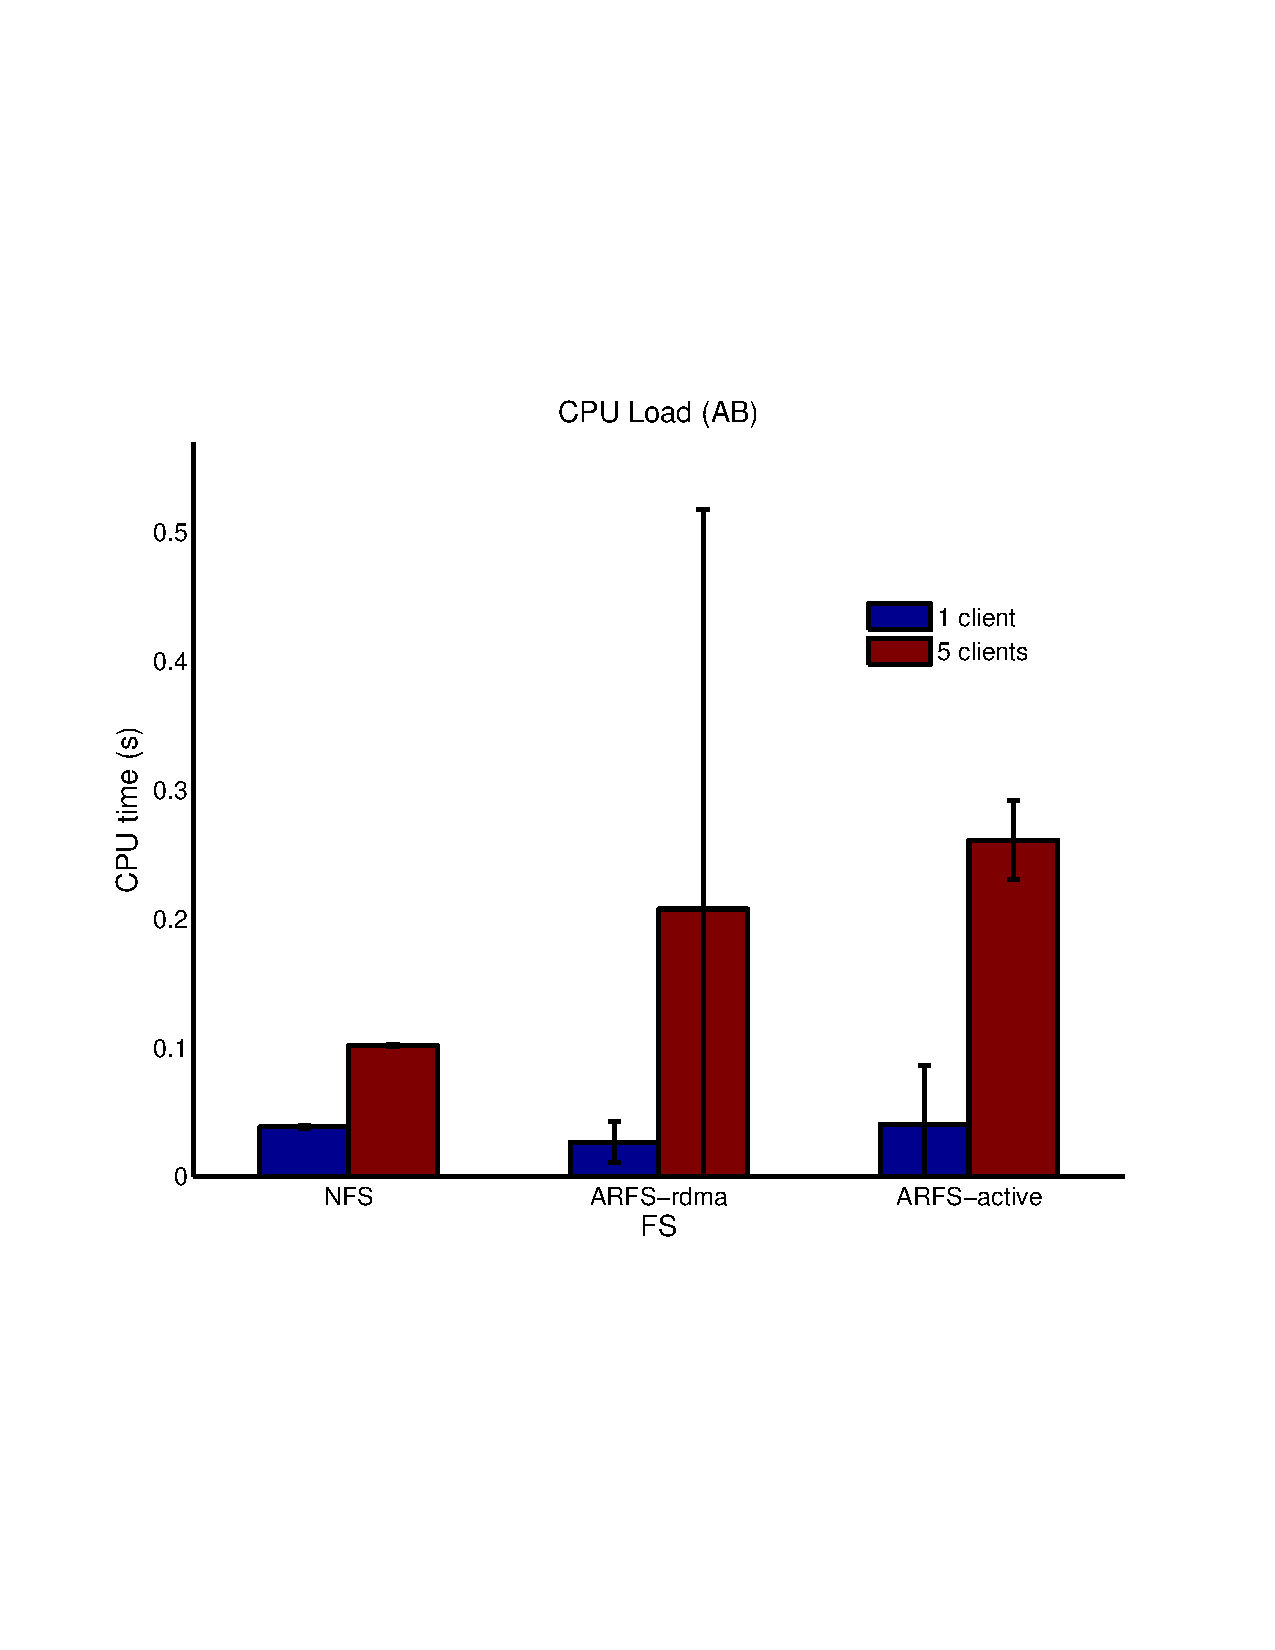
\includegraphics[scale=0.5, trim = 0 200 0 200]{../../results/matlab/cpuload.pdf}
  \caption{cpu load}\label{cpuload}
\end{figure}

\begin{figure}
  \centering
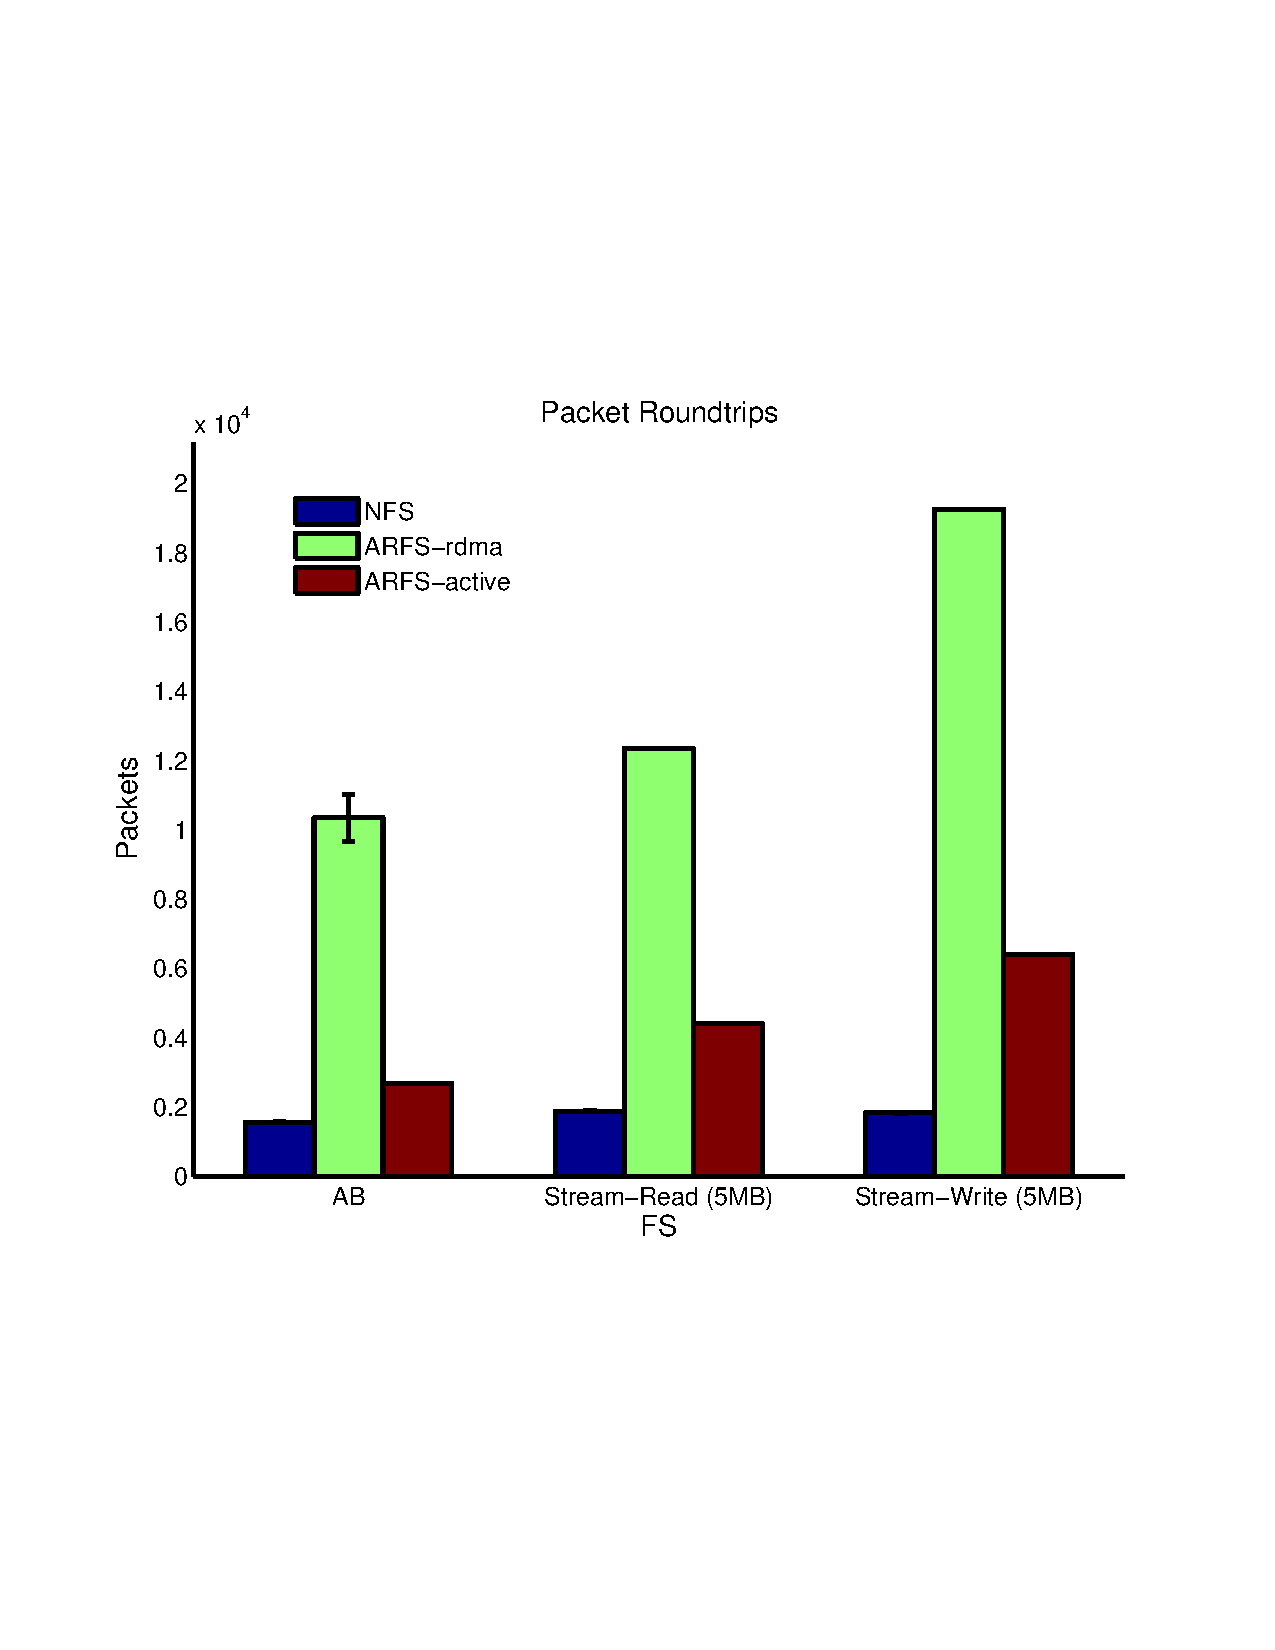
\includegraphics[scale=0.5, trim = 0 200 0 200]{../../results/matlab/rt.pdf}
  \caption{rt}\label{rt}
\end{figure}

\begin{figure}
  \centering
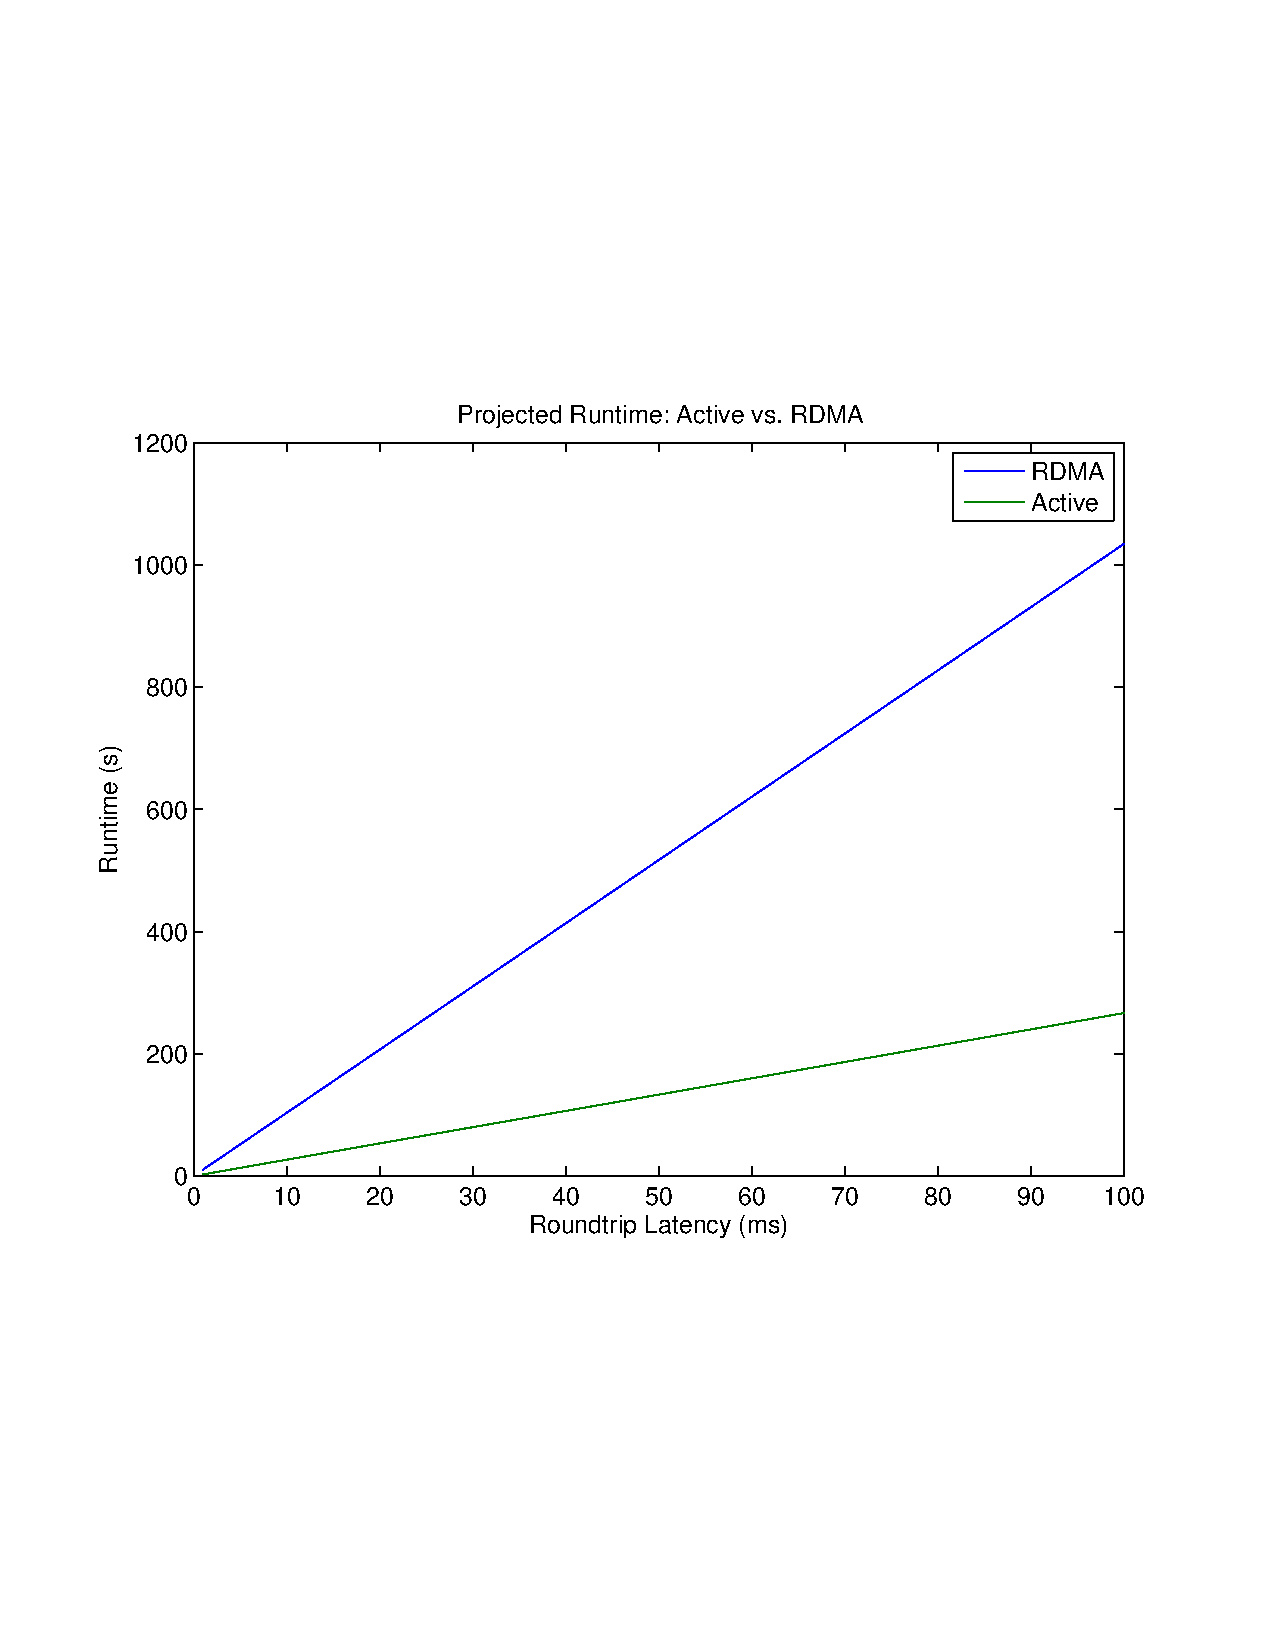
\includegraphics[scale=0.5, trim = 0 200 0 200]{../../results/matlab/synth_time.pdf}
  \caption{synth time}\label{synth_time}
\end{figure}

\begin{figure}
  \centering
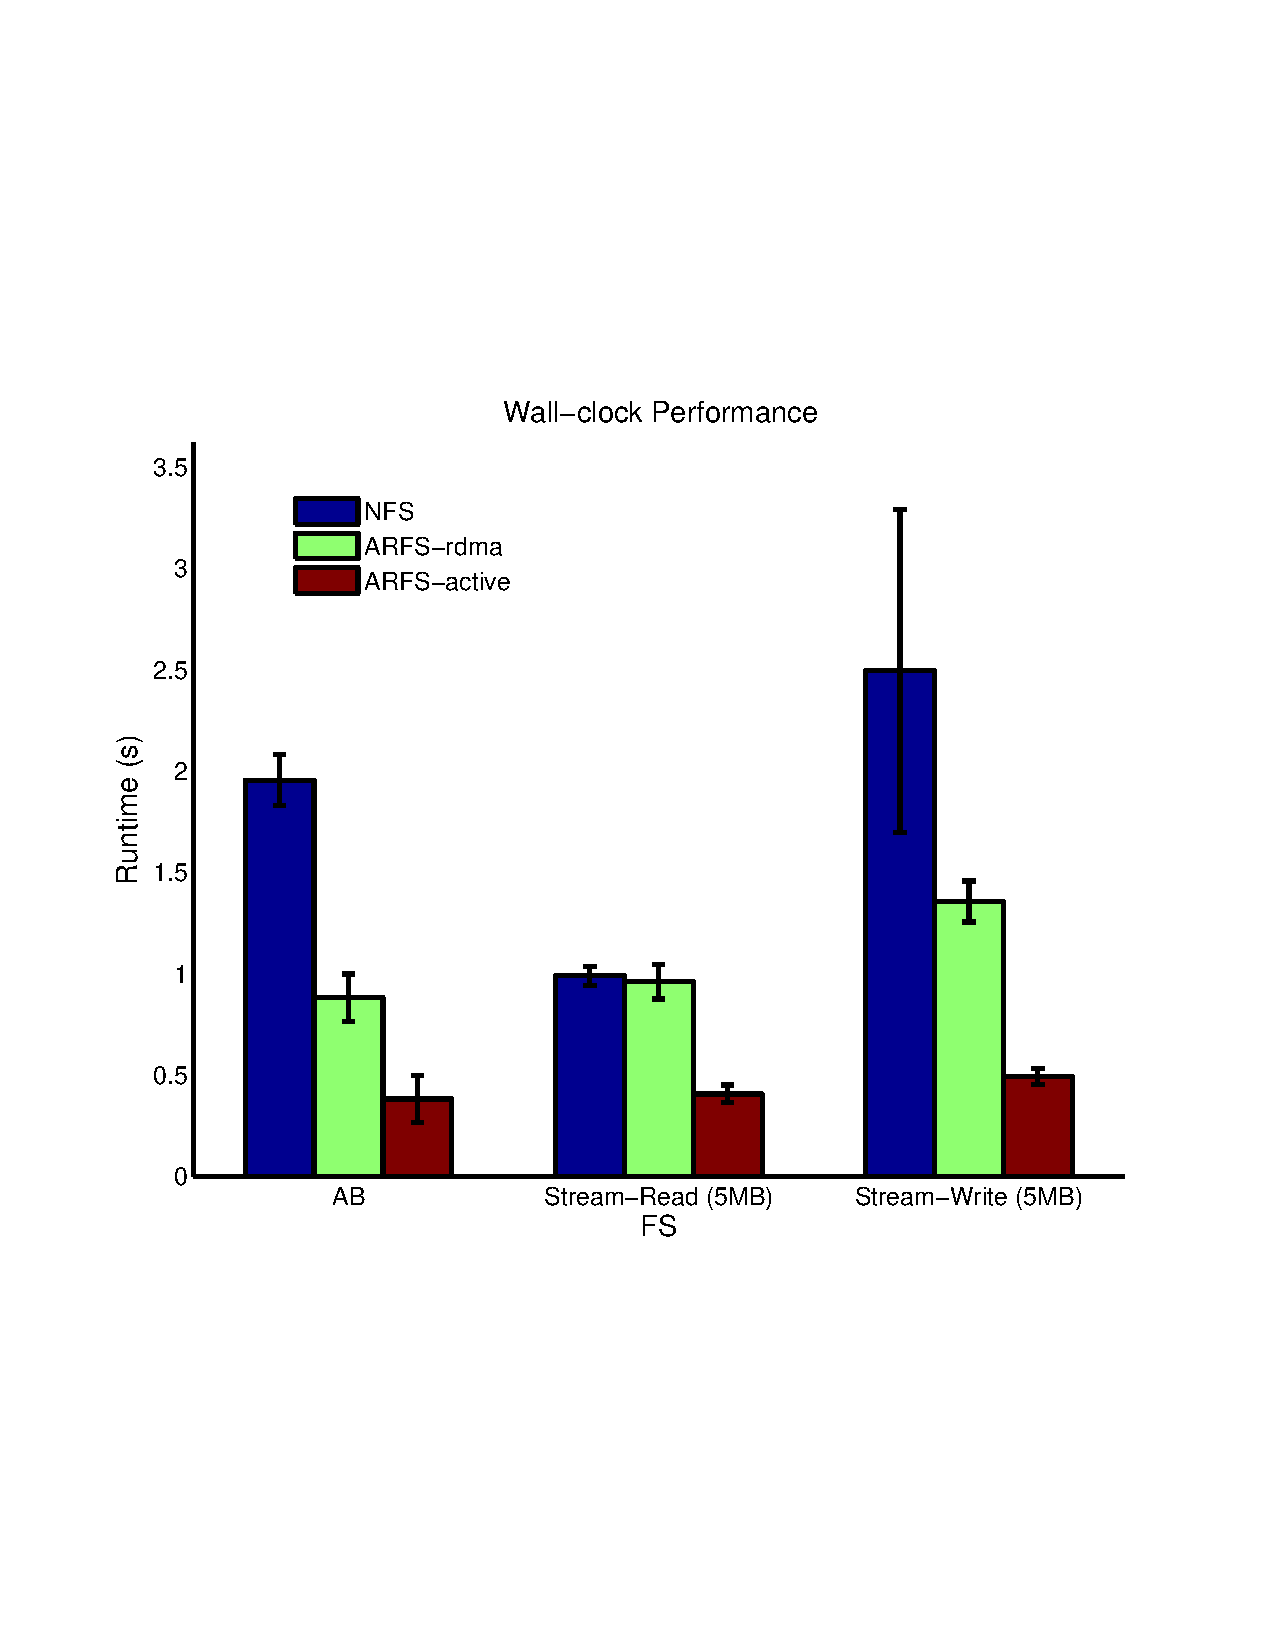
\includegraphics[scale=0.5, trim = 0 200 0 200]{../../results/matlab/wallclock.pdf}
  \caption{wallclock}\label{wallclock}
\end{figure}

\begin{figure}
  \centering
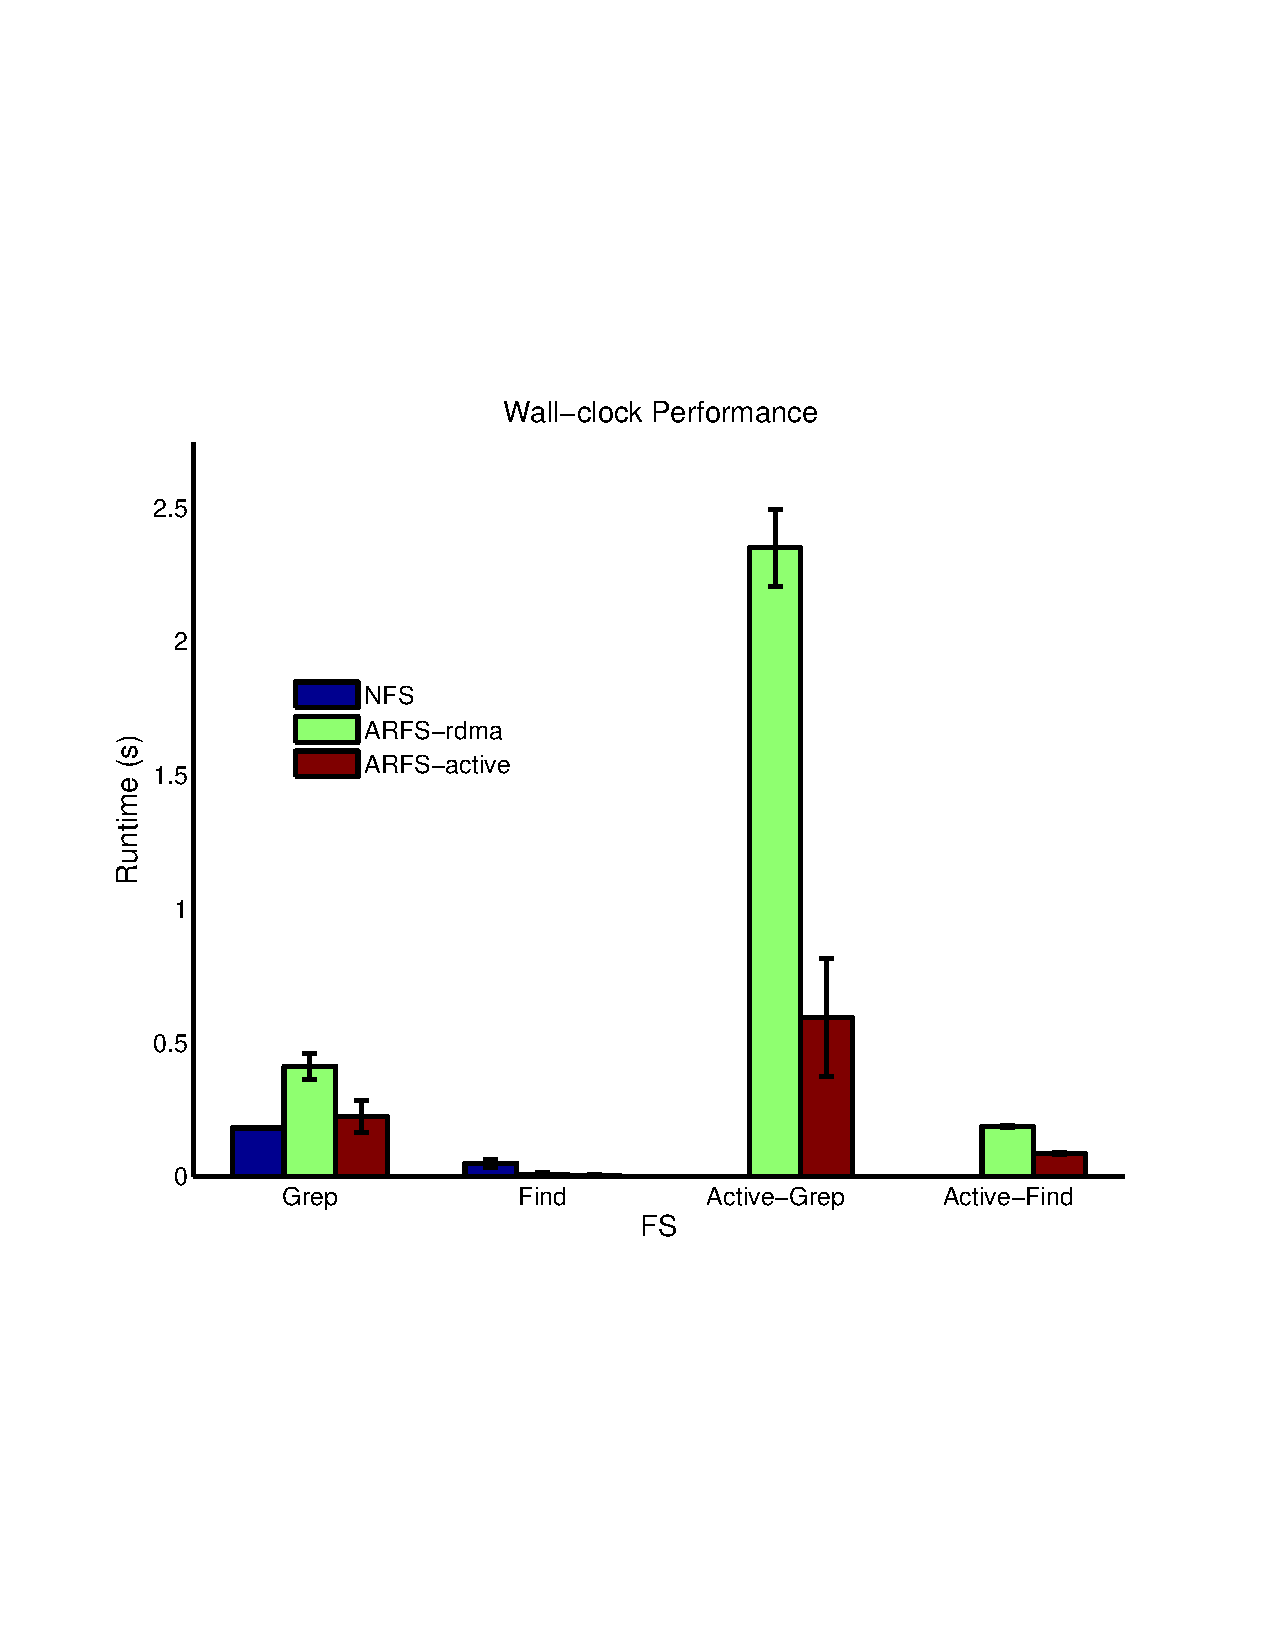
\includegraphics[scale=0.5, trim = 0 200 0 200]{../../results/matlab/wallclock2.pdf}
  \caption{wallclock2}\label{wallclock2}
\end{figure}

\section{Future Work}
\begin{itemize}
\item Evaluate the system with a real system with a real network card with
a real coprocessor running the JVM. Go even further, and implement the code
on the NIC GPU. This will enable better comparison with NFS.
\item Address scalability issues because NIC processing power limitation, by may
be experimenting with larger number of NIC cards, and evaluating the performance
as a function of cost.
\end{itemize}

\section{Conclusion}
THE WORLD WILL NEVER BE THE SAME AGAIN ;)


\bibliography{final} \bibliographystyle{abbrv}

\end{document}
